\chapter{Results}
\label{ch:Results}
\lettrine[lraise=-0.1, lines=2, loversize=0.2]{T}{his} chapter discusses the experiments carried out to validate the software layer built. The simulation software used for the tests was Gazebo. The simulation environment consists of a high-voltage tower and an operator standing on the ground next to the tower, but as the low-level controllers have all been faked, not much attention has been paid to the simulation elements during the development of the tests. Instead, the focus is on the task distribution and the execution of the \glspl{BT}.

The experiments were divided into two phases. In the first phase, simulations involving a single \gls{ACW} were carried out in order to test the performance of each element of the system in a controlled manner. On the one hand, it was checked that the \emph{High-Level Planner} performed the mission planning correctly, assigning the tasks as expected according to the specifications and constraints, and on the other hand, it was checked that the \emph{Agent Behaviour Manager} performed its function correctly, both the execution of individual tasks and the ability to detect and act in case of unforeseen events. During this phase, the validation of the distributed block takes centre stage.

In the second phase, the simulations consisted of including multiple \glspl{ACW} and testing in different scenarios. This phase focuses less on validating the \gls{BT}, which would be fully validated during the first phase, and more on evaluating the capabilities of the \emph{High-Level Planner}. The situations faced by the system in this phase involve disconnections, reconnections, input of new tasks, modifications of the battery level, etc. In addition, the type of \glspl{ACW} has been modified from one test to another. Since the \glspl{BT} are fully validated at this stage, the visualisation of the simulation in Gazebo is not as important. That is why the results of this phase are mostly presented by visualising the \glspl{BT} with the Groot tool and by means of the information printed by both blocks through the terminal. 

\section{Phase I: single ACW simulations}
\label{sec:phaseI}
Once the simulation has finished initialising, tasks can start to be requested. To do so, the fake \emph{Gesture Recognition} block has to be executed indicating the type and parameters of the task. As the simulations during this phase consist of a single \gls{ACW}, the behaviour of the planner is quite predictable, so in addition to validating the \gls{BT}, these tests can be used to make a first verification of the \emph{High-Level Planner} block.

First, a series of tasks were requested and executed without interruption in order to check that the system worked well under favourable conditions and was able to complete all tasks. Next, the responsiveness of the \emph{Agent Behaviour Manager} block to unforeseen events was evaluated. In this part the behaviour of the planner remained predictable without the need for any calculations. It started by requesting, in that order, a \emph{Tool Delivery} task, an \emph{Inspection} task and a \emph{Safety Monitoring} task. The expected order in which the tasks will be assigned is the same order.

\begin{figure}[htbp]
    \centering
    \subfloat[Starting position of the Gazebo simulation]{
        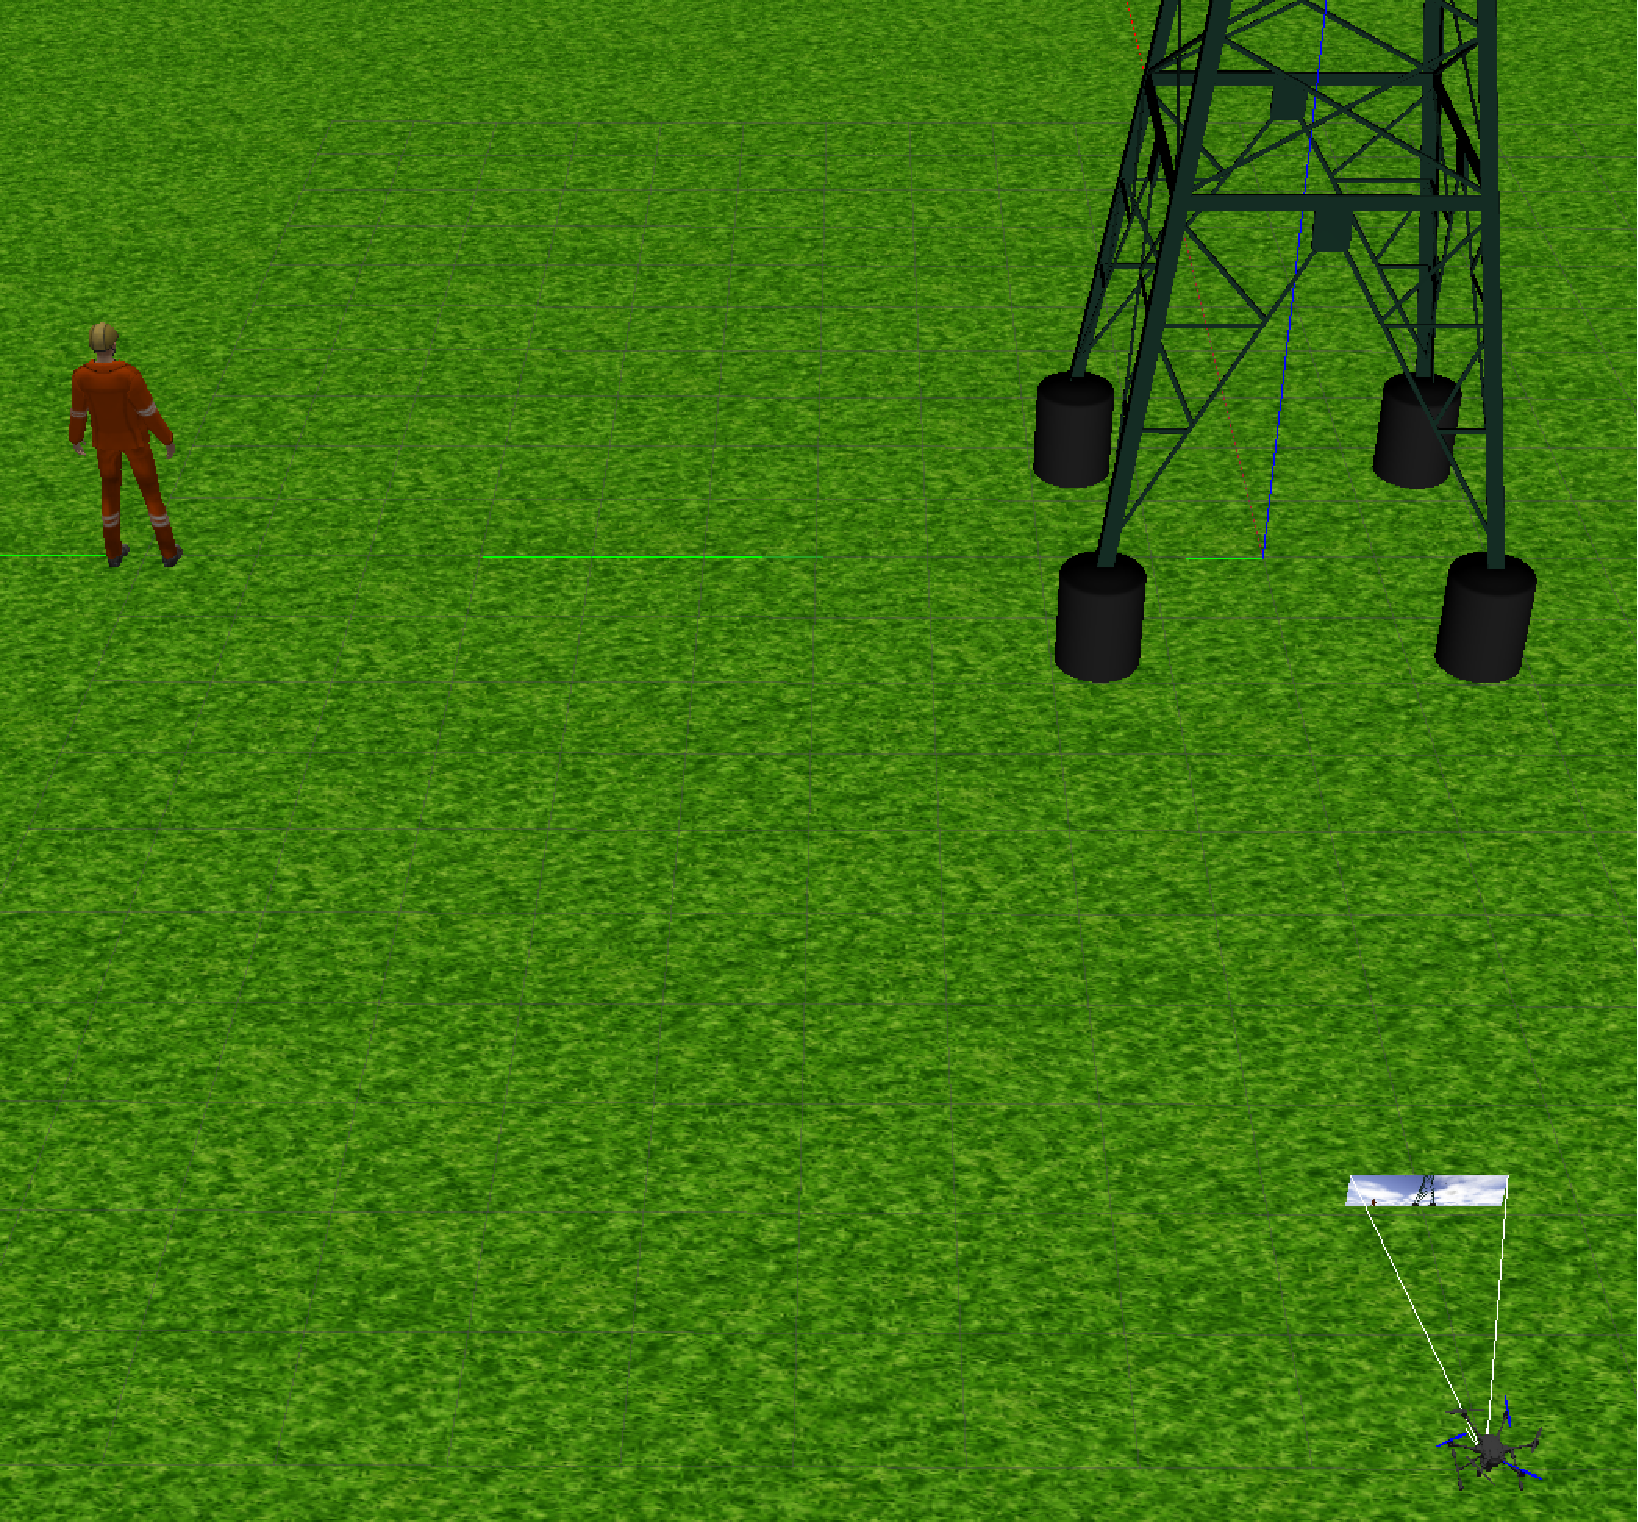
\includegraphics[width=.45\linewidth]{Results/figures/GazeboBatSta.pdf}}
    \hfill
    \subfloat[\gls{BT}'s starting status displayed with Groot]{
        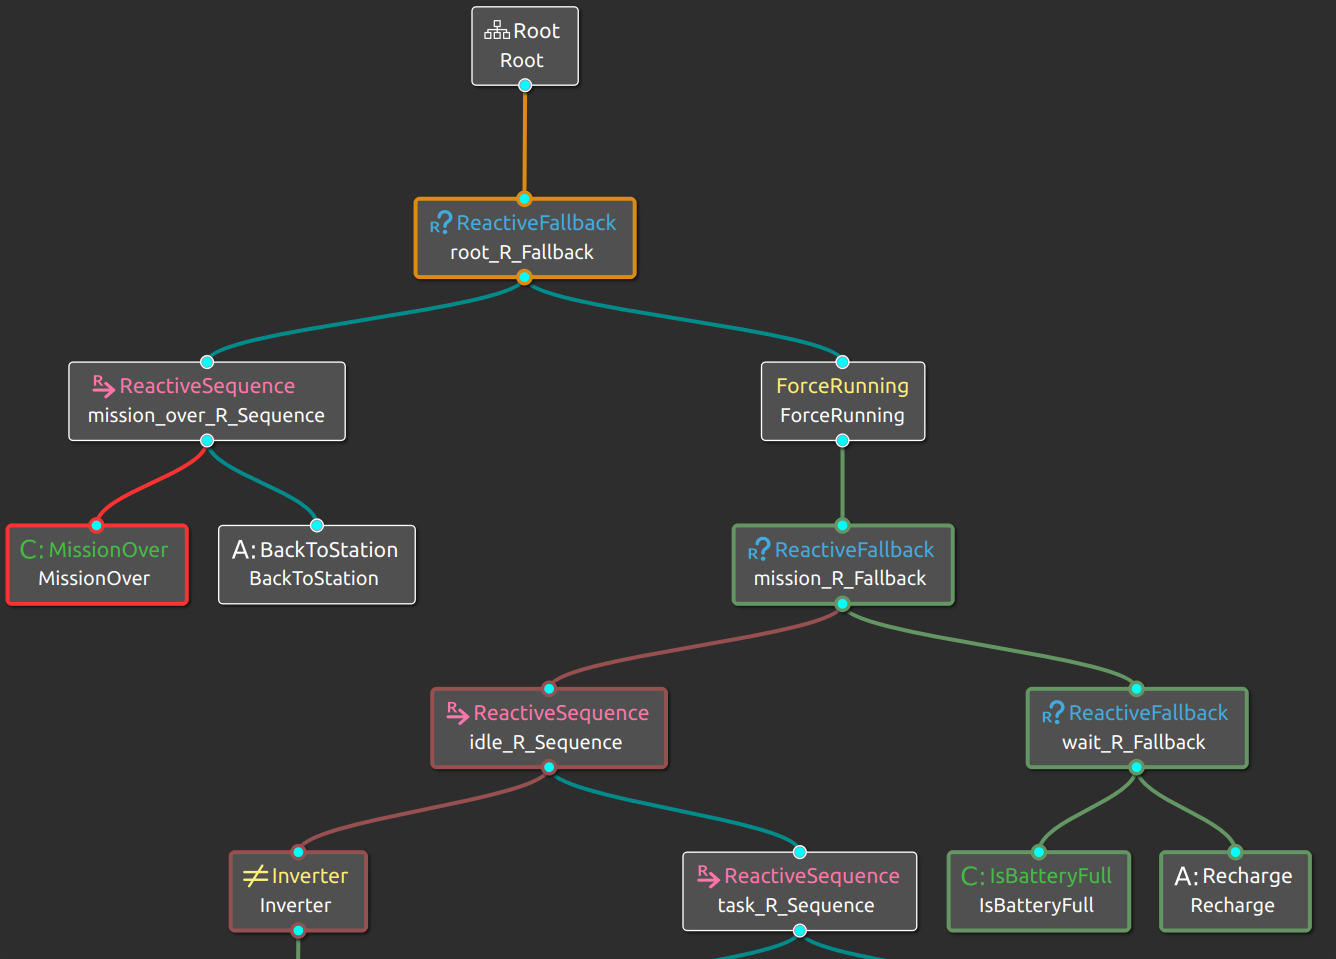
\includegraphics[width=.45\linewidth]{Results/figures/BTini.jpeg}}
    \caption{Initial status of the simulation: battery charged and no task queued.}
    \label{fig:BTinitialization}
\end{figure}

At the beginning, the \gls{UAV} has the battery charged, is landed on the charging station and has no task queued, then the \gls{BT} is returning \emph{SUCCESS} except for the \emph{Force Running} node, which keeps the \gls{BT} running by always returning \emph{RUNNING} (see Fig. \ref{fig:BTinitialization}). Note that Groot uses its own colour code to represent the result of each node in the previous tick. \emph{Green} stands for \emph{SUCCESS}, \emph{Red} for \emph{FAILURE}, \emph{Orange} for \emph{RUNNING} and \emph{White} for \emph{IDLE}. In addition, when a node is still called by a \emph{Reactive Control} node after it has finished, if the result is the same, the colour of the node is maintained but in a less intense tone. 

\begin{figure}[htbp]
    \centering
    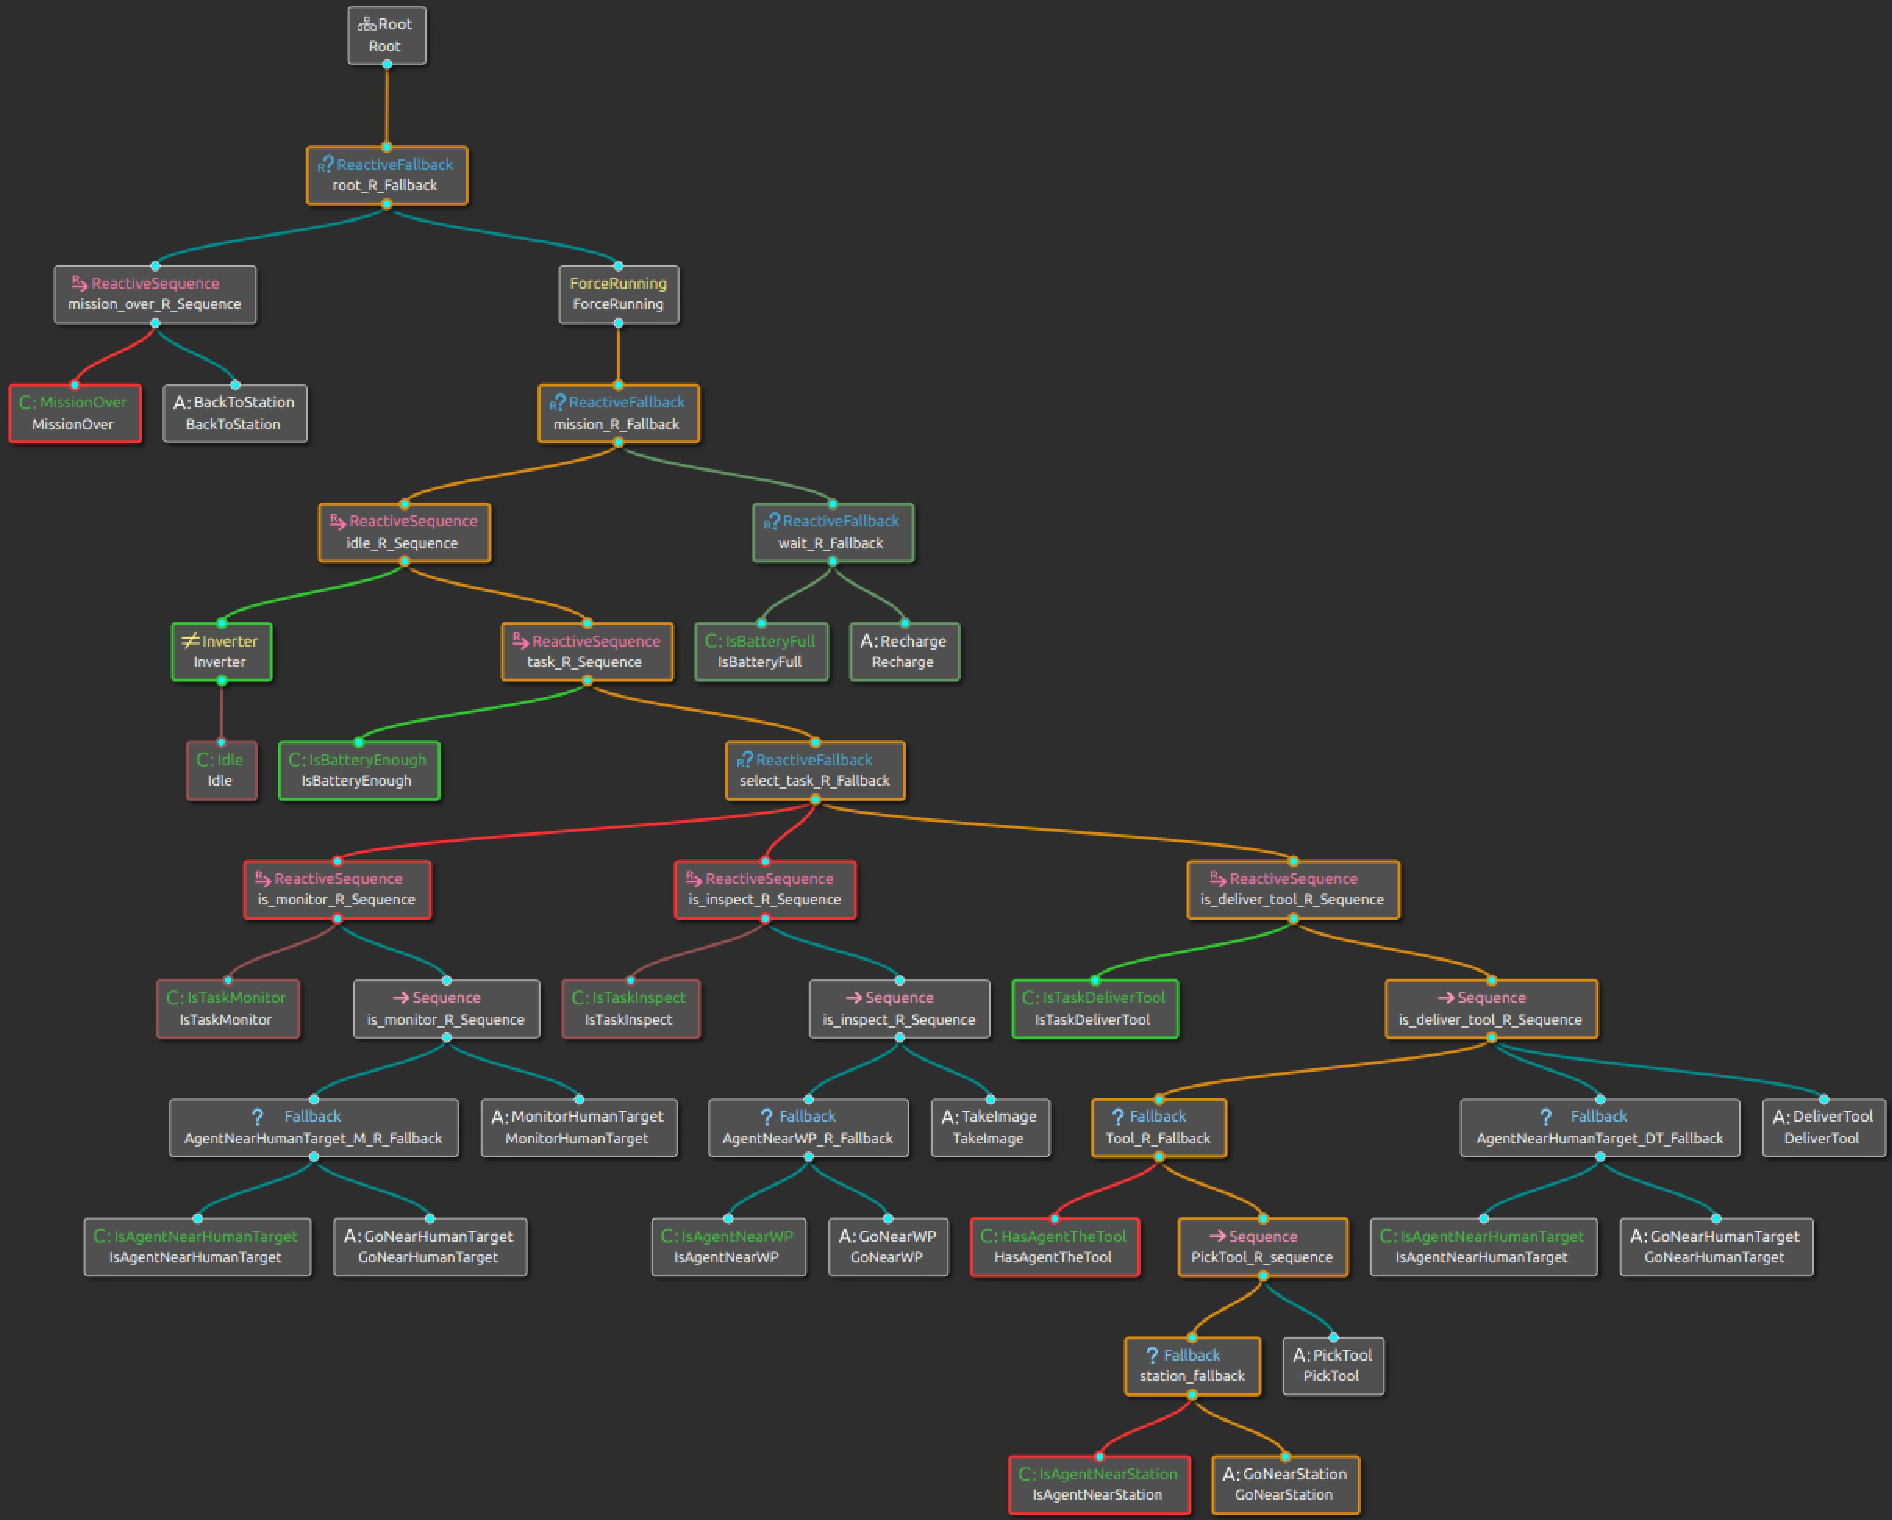
\includegraphics[width=.75\linewidth]{Results/figures/BTnoIdle.pdf}
    \caption{\gls{BT} transition from idle to \emph{Tool Delivery Task Tree}}
    \label{fig:NoIdle_DeliverToolTaskTree}
\end{figure}

Once the first task arrives the \gls{ACW} starts running. The \gls{BT} now checks which task it is and proceeds with its execution (see Fig. \ref{fig:NoIdle_DeliverToolTaskTree}). At this point the other two tasks were communicated. The \emph{High-Level Planner} performed a replanning for each event, but as the \emph{Tool Delivery} task remained at the top of the queue, the \gls{BT} did not notice the change. Figure \ref{fig:newtaskqueue} shows both the mentioned replanning and the parameters selected by the planner for each of the tasks.

% \ref{fig:newtaskqueue}: Captura del terminal para ver las comunicaciones y las replanificaciones hasta este punto
\begin{figure}[htbp]
    \centering
    \includegraphics[width=.75\linewidth]{Results/figures/prov.jpeg}
    \caption{Feedback of the task planning process and communications between \emph{High-Level Planner} and \emph{Agent Behaviour Manager}}
    \label{fig:newtaskqueue}
\end{figure}

The \emph{Tool Delivery Task Tree} functioned perfectly well. In Gazebo, the movement of the \gls{ACW} from one side to the other was observed as the \gls{BT} traversed the nodes of the subtree of this task (see Fig. \ref{fig:Gazebo_DeliverTree}). In addition, the task result was checked for correct communication with the centralised block, which used the moment to re-evaluate the plan to see if it is still within the optimal plan. As the plan did not change, the \gls{BT} continued to execute the queued tasks. As it has already been shown that the activation of \emph{Action} nodes in the \gls{BT} correctly moves the \gls{ACW} in the Gazebo simulation, no screenshots of the simulation are shown from now on as they are not relevant. Figure \ref{fig:Gazebo_InspectTree} shows the evolution of the \gls{BT} during the execution of the \emph{Inspection} task, for which the \gls{BT} also proved to work perfectly. 

\begin{figure}[htbp]
    \centering
    \subfloat[Initial position: charge station]{
        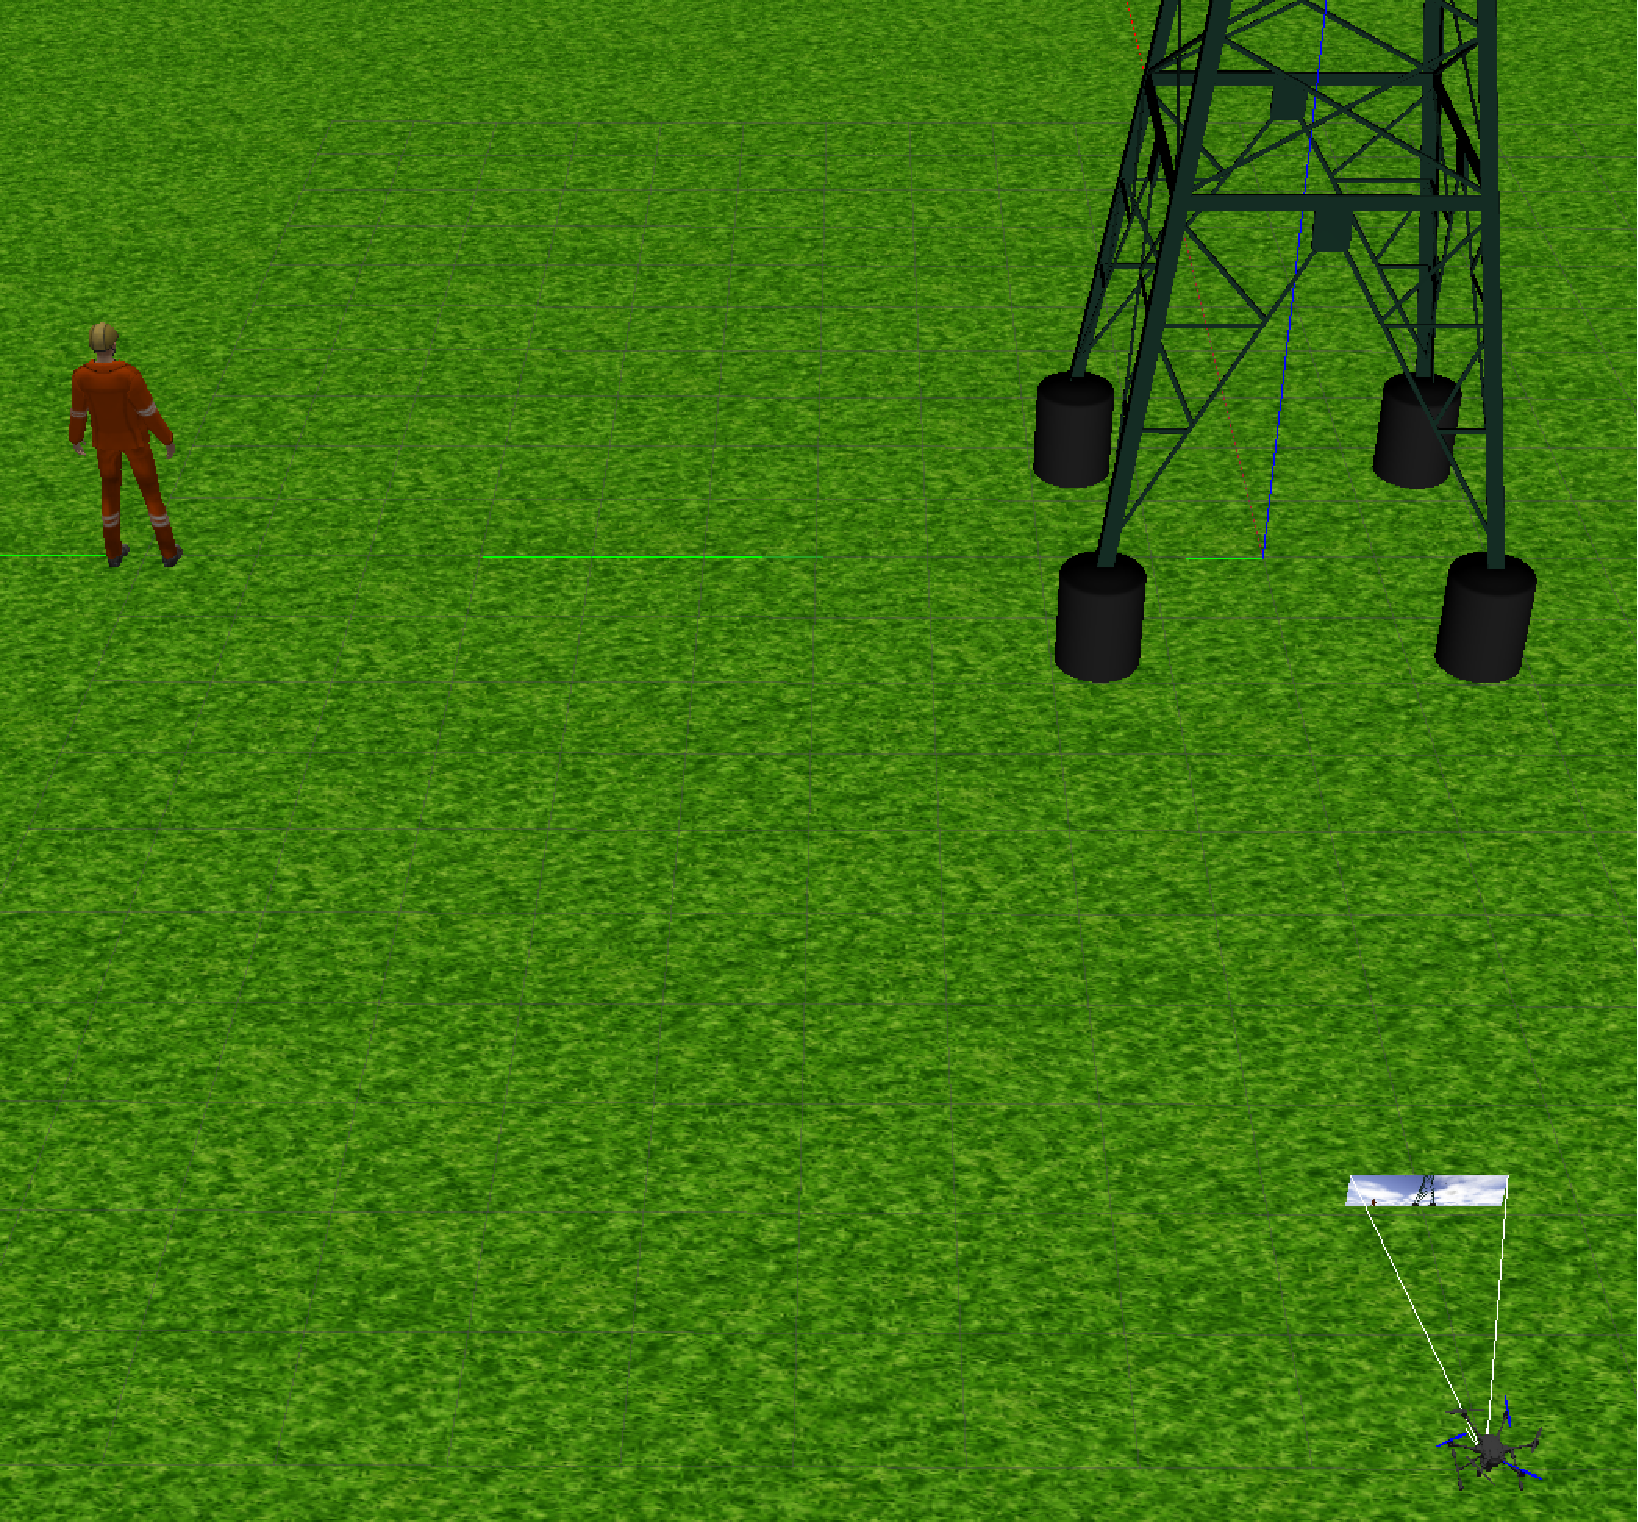
\includegraphics[width=.3\linewidth]{Results/figures/GazeboBatSta.pdf}}
    \hfill
    \subfloat[Base station: tool picking]{
        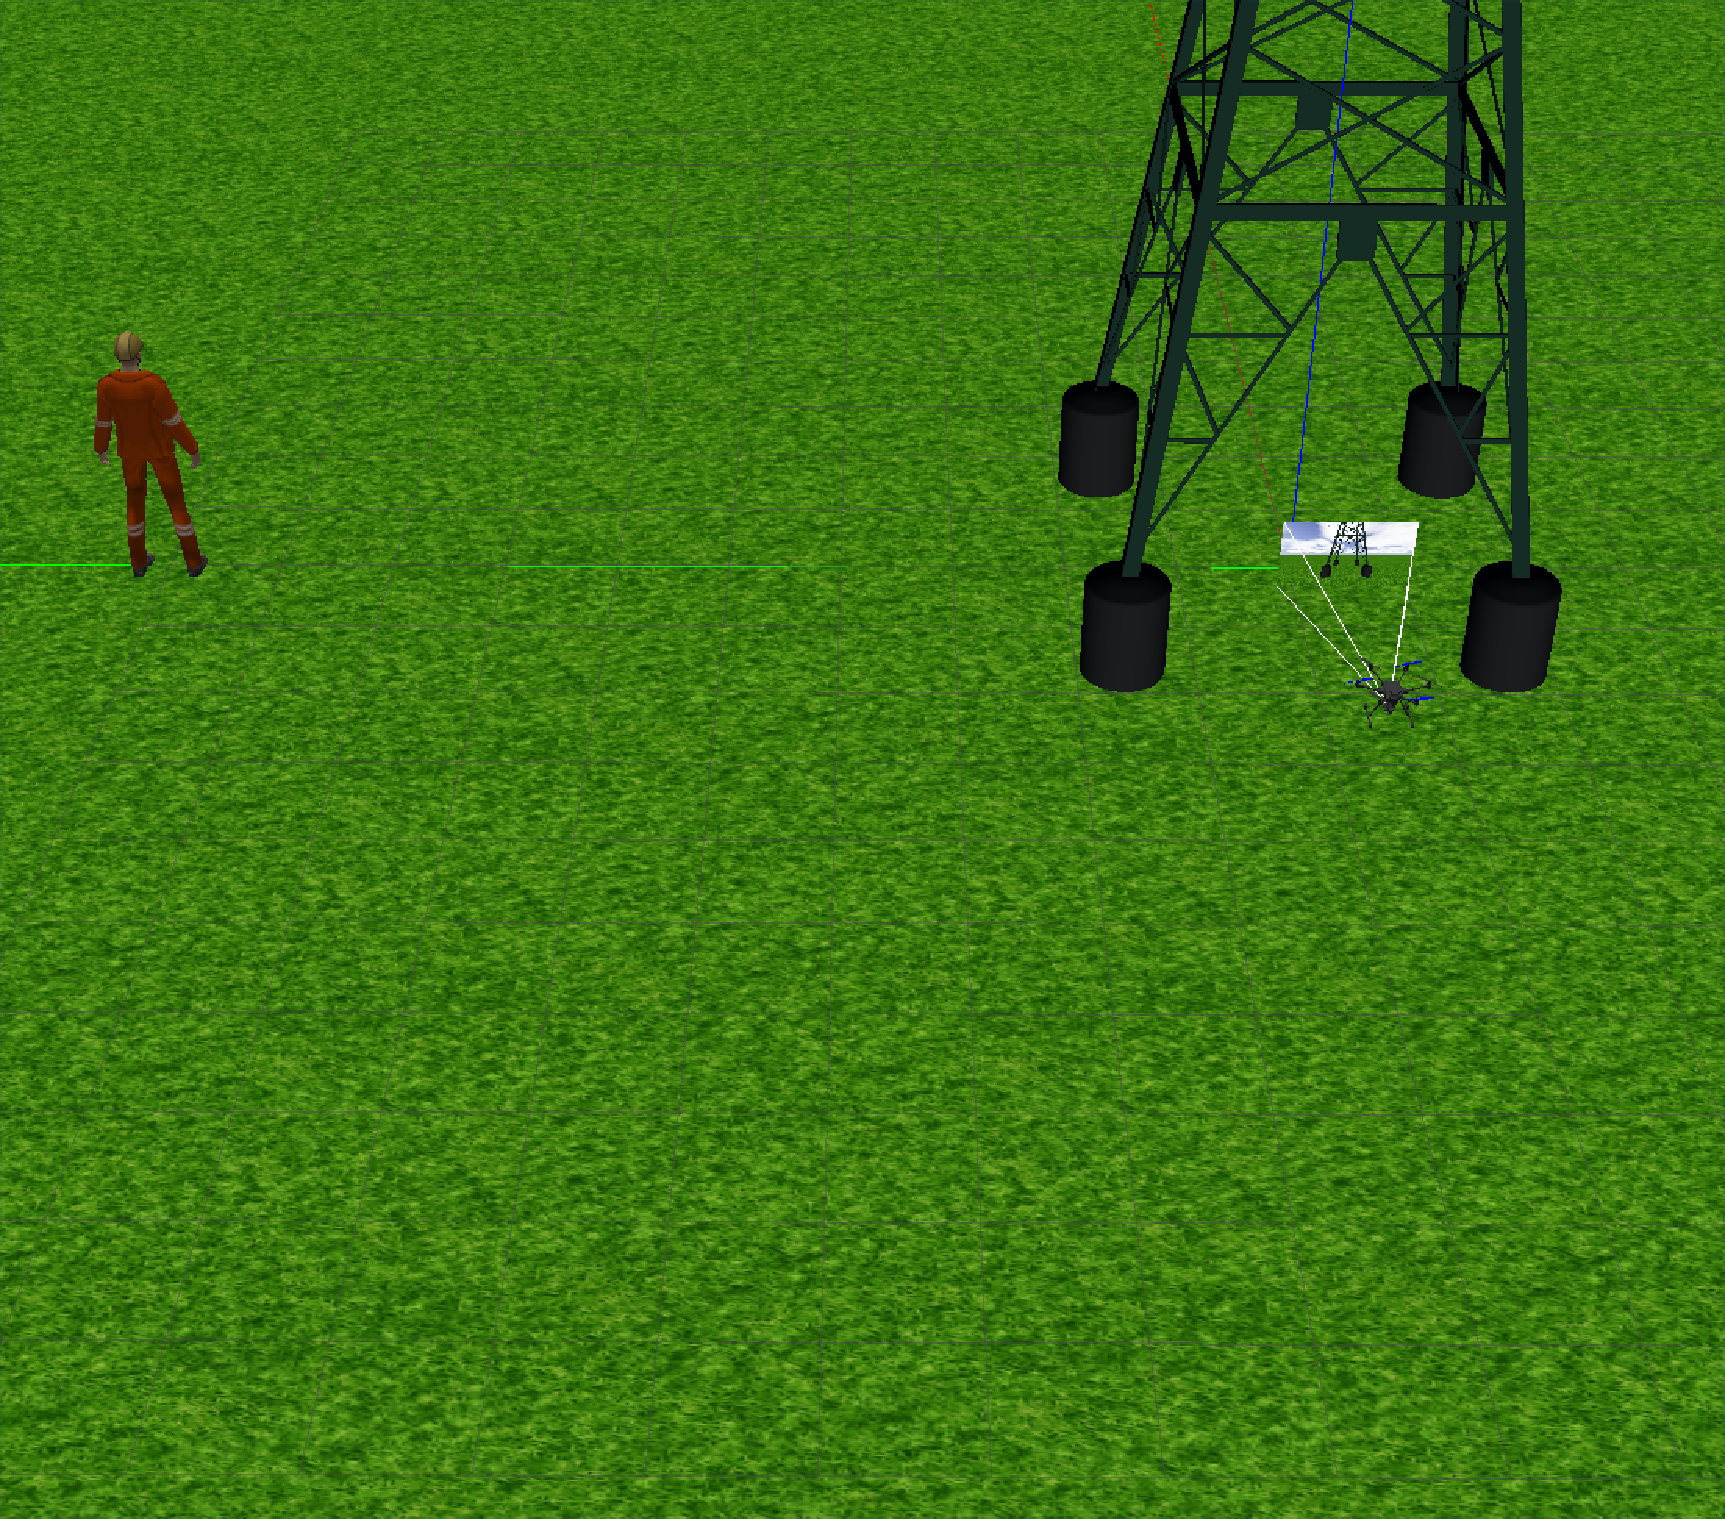
\includegraphics[width=.3\linewidth]{Results/figures/GazeboTool.pdf}}
    \hfill
    \subfloat[Human target position: tool delivery]{
        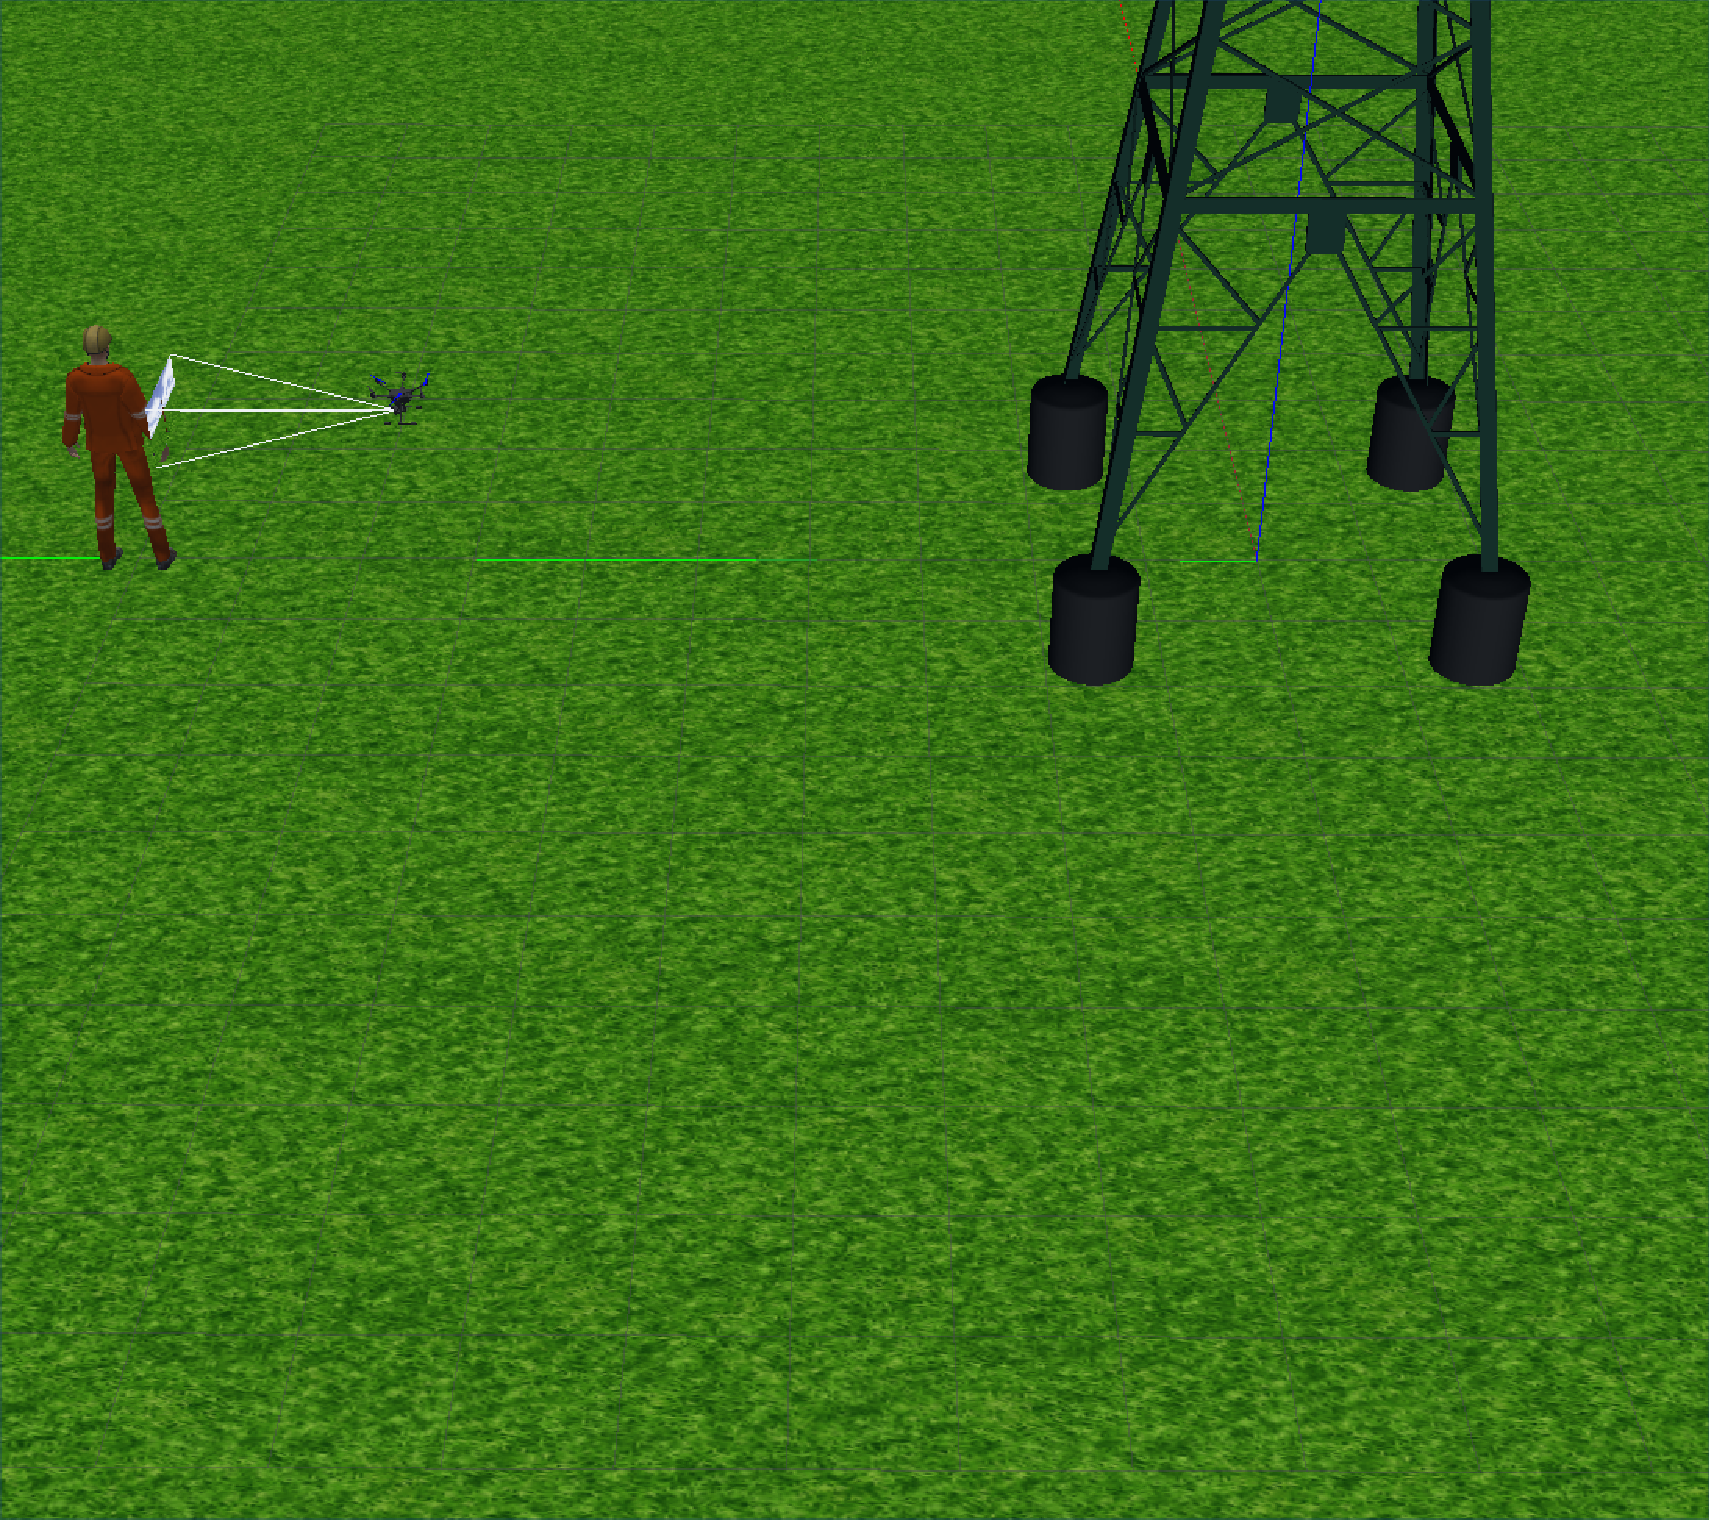
\includegraphics[width=.3\linewidth]{Results/figures/GazeboHuman.pdf}}
    \hfill
    \\
    \subfloat[Activation of \emph{Go Near Station} action after checking \emph{Has ACW the tool?} and \emph{Is ACW near Station?} conditions]{
        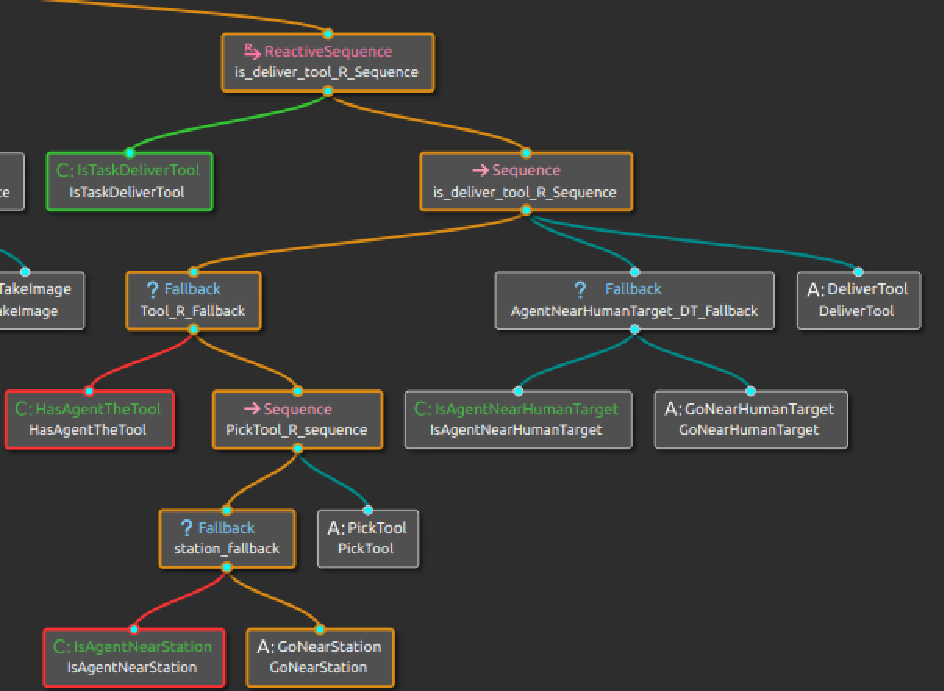
\includegraphics[width=.45\linewidth]{Results/figures/BTDTGNS.pdf}}
    \hfill
    \subfloat[Activation of \emph{Pick Tool} action after arriving at the base station]{
        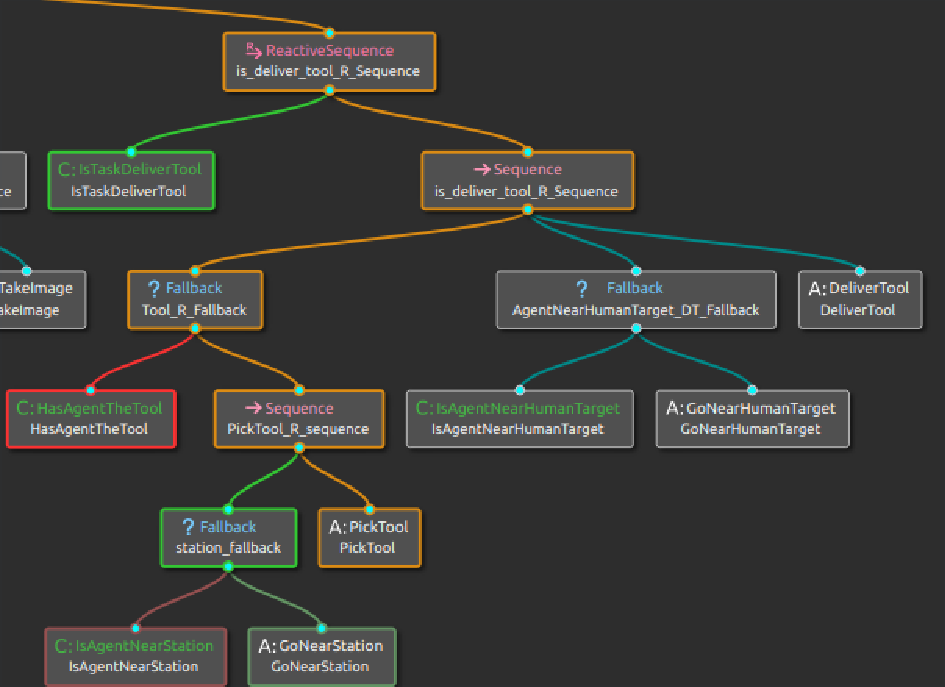
\includegraphics[width=.45\linewidth]{Results/figures/BTDTPT.pdf}}
    \\
    \subfloat[Activation of \emph{Go Near Human Target} action after having the tool and checking \emph{Is ACW Human Target?} condition]{ 
        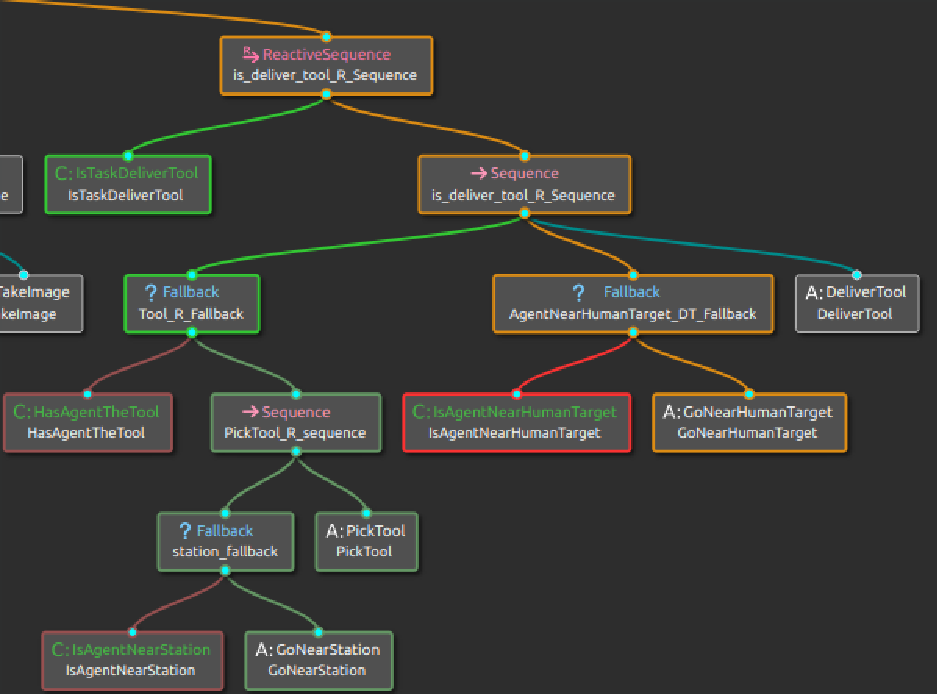
\includegraphics[width=.45\linewidth]{Results/figures/BTDTGNHT.pdf}}
    \hfill
    \subfloat[Activation of \emph{Deliver Tool} action after arriving near human target having the tool]{
        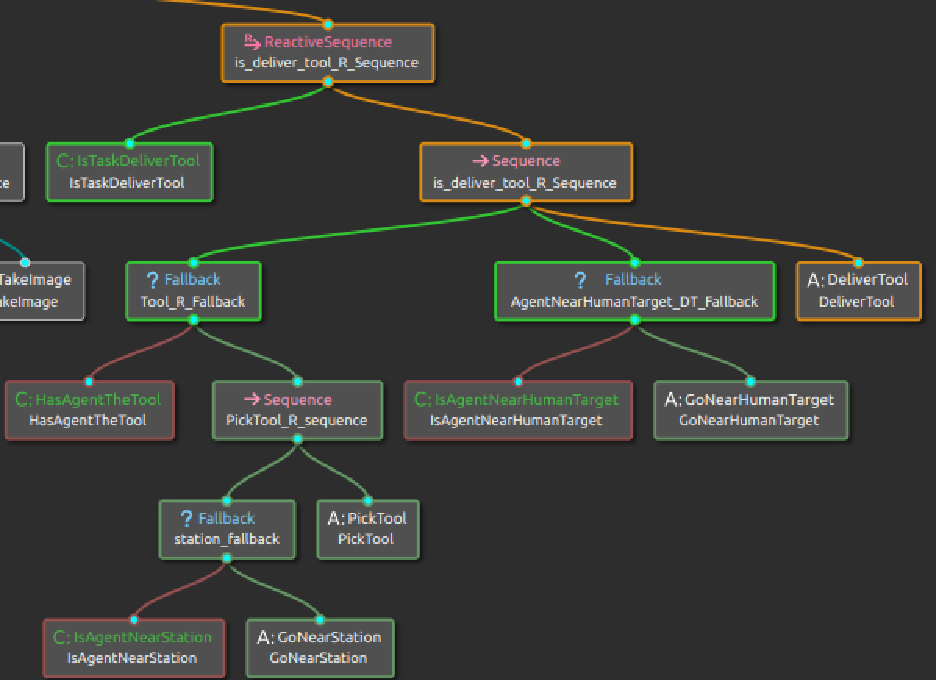
\includegraphics[width=.45\linewidth]{Results/figures/BTDTDT.pdf}}
    \caption{Evolution of the simulation during the execution of the \emph{Tool Delivery Task Tree}}
    \label{fig:Gazebo_DeliverTree}
\end{figure}

\begin{figure}[htbp]
    \centering
    \subfloat[Activation of \emph{Go Near WP} action after checking \emph{Is Agent Near WP?} condition]{
        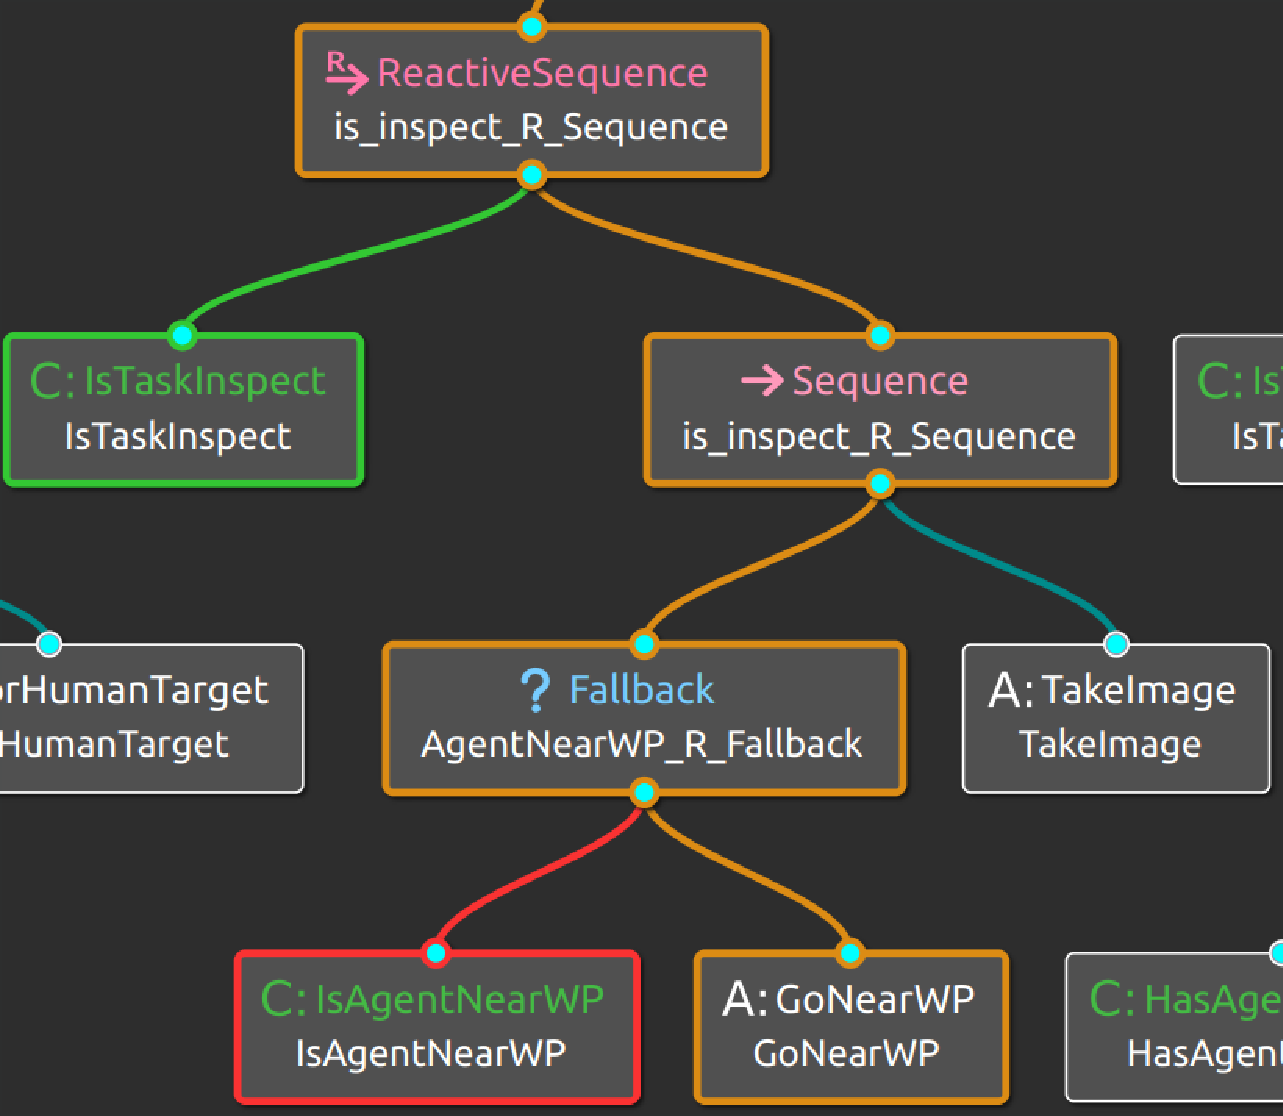
\includegraphics[width=.45\linewidth]{Results/figures/BTIGNWP.pdf}}
    \hfill
    \subfloat[Activation of \emph{Take Image} action after arriving near WP]{
        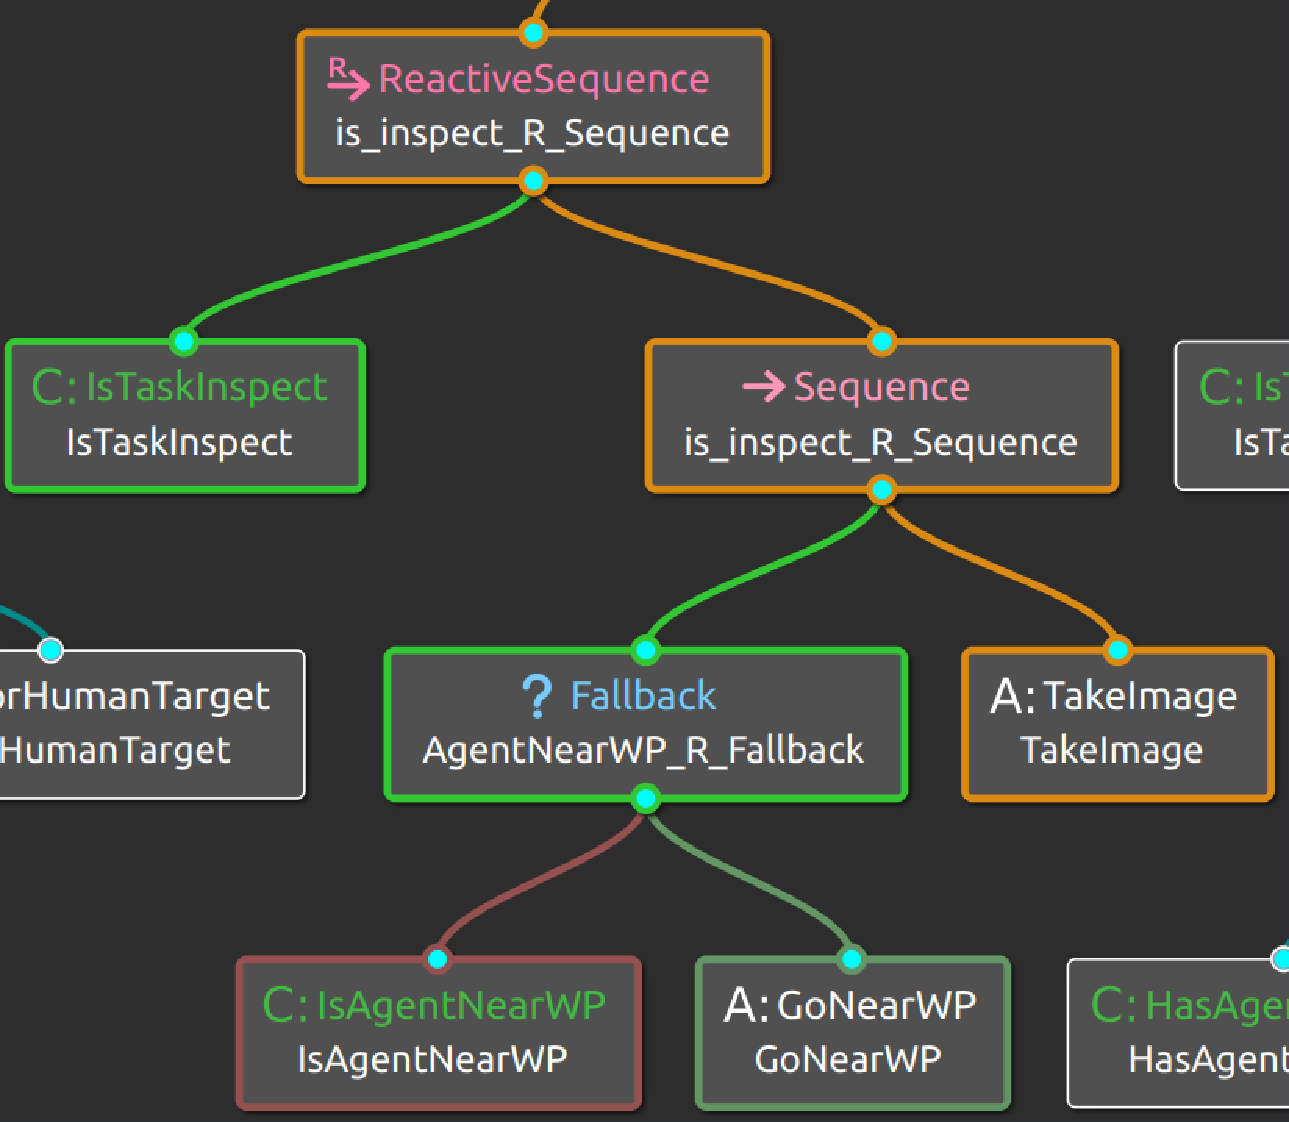
\includegraphics[width=.45\linewidth]{Results/figures/BTITI.pdf}}
    \caption{Evolution of the \gls{BT} during the execution of the \emph{Inspection Task Tree}}
    \label{fig:Gazebo_InspectTree}
\end{figure}

Finally, when this task was finished, the \gls{BT} proceeded to execute the \emph{Safety Monitoring} task, which was also carried out without problems (see Fig. \ref{fig:Gazebo_MonitorTree}). This task ends when the operator requests it, so the fake block pretending to be the low-level controller for this task is programmed so that the task never ends. This task remains in the queue until the mission is completed or it is overwritten by a task of another type with the same \gls{ID}, which is a contemplated case for which the planner is prepared and warns the operators that an unfinished task is going to be deleted. Since during planning, tasks are assigned in order, the non-completion of this task is not a problem for the execution of other tasks, but an opportunity to study in a controlled way the emergency protocols and the response of both blocks to different unforeseen events.

\begin{figure}[htbp]
    \centering
    \subfloat[Activation of \emph{Go Near Human Target} action after checking \emph{Is Agent Near Human Target?} condition]{
        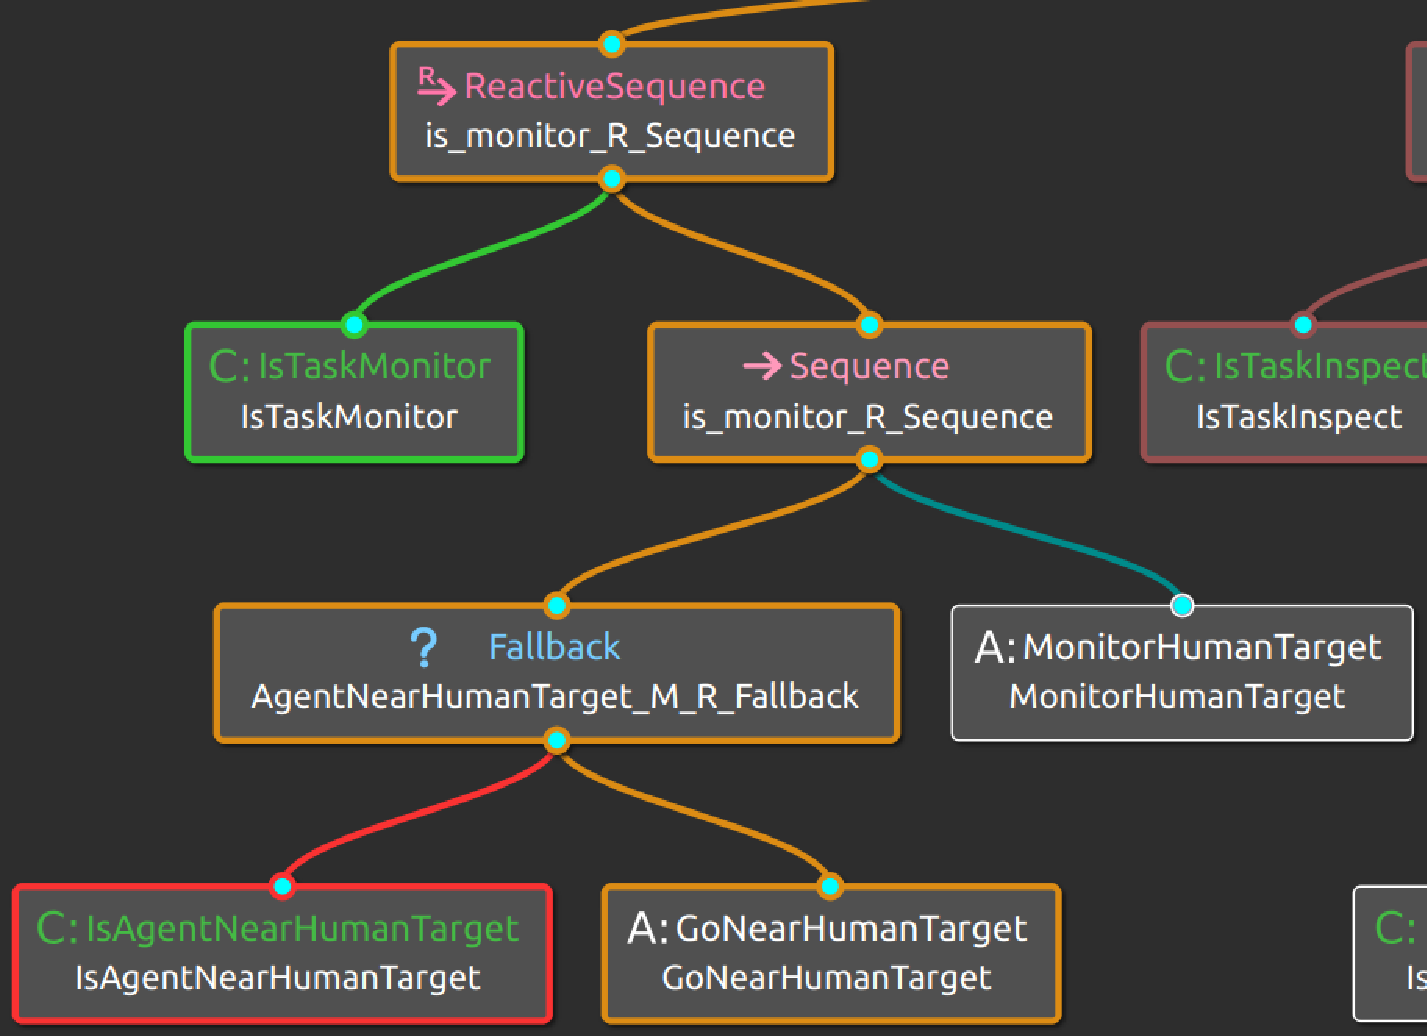
\includegraphics[width=.45\linewidth]{Results/figures/BTMGNHT.pdf}}
    \hfill
    \subfloat[Activation of \emph{Monitor Human Target} action after arriving near Human Target]{
        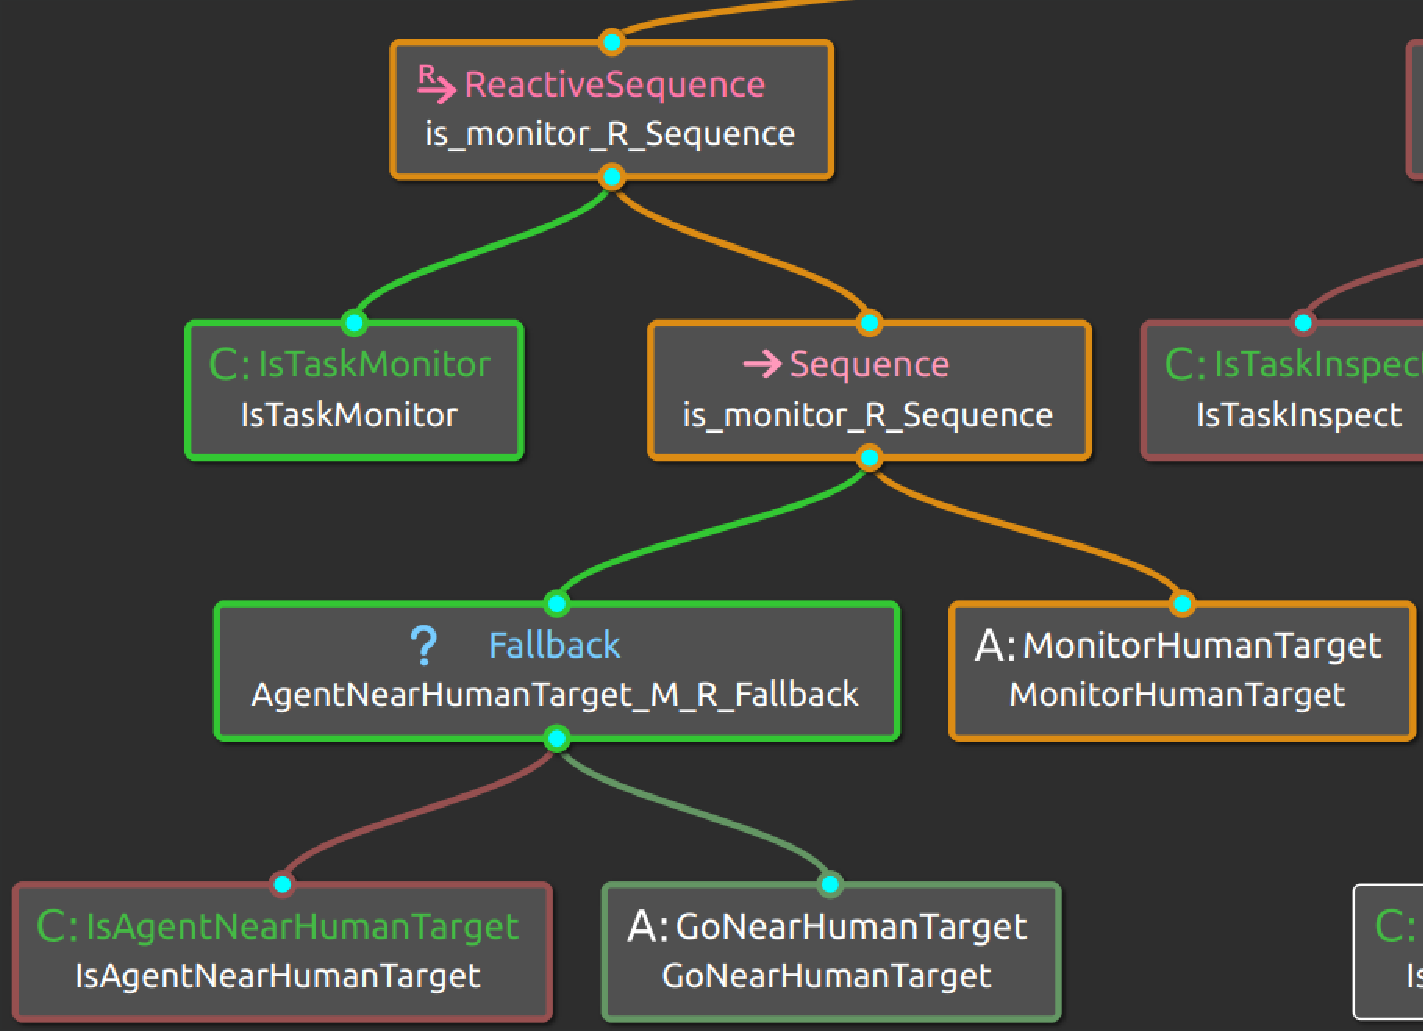
\includegraphics[width=.45\linewidth]{Results/figures/BTMMHT.pdf}}
    \caption{Evolution of the \gls{BT} during the execution of the \emph{Monitoring Task Tree}}
    \label{fig:Gazebo_MonitorTree}
\end{figure}

Once it had been verified that the system worked well in the absence of unforeseen events, the system was tested in all kinds of situations. First, the \gls{BT}'s ability to stop the current task and switch to the execution of the new task in the event of a change of plans was tested. This was done by first requesting a \emph{Safety Monitoring} task and then requesting a \emph{Tool Delivery} task, which, having a higher priority, will move the previous task from the top of the queue. Figure \ref{fig:event_ChangeOfPlans} shows the communications performed during this process, the movement of the \gls{ACW} in the simulation, and the evolution of the \gls{BT}.

% \ref{fig:event_ChangeOfPlans}: Evolución del BT (groot), mensajes del terminal y capturas de Gazebo durante un cambio de planes.
\begin{figure}[htbp]
    \centering
    \subfloat[]{ % <- Caption
        \includegraphics[width=.45\linewidth]{Results/figures/prov.jpeg}}
    \hfill
    \subfloat[]{ % <- Caption
        \includegraphics[width=.45\linewidth]{Results/figures/prov.jpeg}}
    \\
    \subfloat[]{ % <- Caption
        \includegraphics[width=.45\linewidth]{Results/figures/prov.jpeg}}
    \hfill
    \subfloat[]{ % <- Caption
        \includegraphics[width=.45\linewidth]{Results/figures/prov.jpeg}}
    \\
    \subfloat[]{ % <- Caption
        \includegraphics[width=.45\linewidth]{Results/figures/prov.jpeg}}
        \hfill
    \subfloat[]{ % <- Caption
        \includegraphics[width=.45\linewidth]{Results/figures/prov.jpeg}}
    \caption{Evolution of the simulation during a change of plans. \emph{Tool Delivery} task displaces \emph{Safety Monitoring} task}
    \label{fig:event_ChangeOfPlans}
\end{figure}

After the success of the previous test, it was tested whether the \emph{High-Level Planner} is able to handle the situation when a new task with a repeated \gls{ID} arrives. For this purpose, an inspection task with the same \gls{ID} as the previous \emph{Tool Delivery} task was sent before the previous \emph{Tool Delivery} task was finished. The system passed the test successfully as shown in figure \ref{fig:event_DuplicatedID}, the task was cancelled and deleted by the \emph{High-Level Planner}, and the \gls{BT} simply reacted to the change of plans as in the previous situation.

% \ref{fig:event_DuplicatedID} Evolución del BT (groot), mensajes del terminal y capturas de Gazebo durante un cambio de planes por la llegada de una ID repetida
\begin{figure}[htbp]
    \centering
    \subfloat[]{ % <- Caption
        \includegraphics[width=.45\linewidth]{Results/figures/prov.jpeg}}
    \hfill
    \subfloat[]{ % <- Caption
        \includegraphics[width=.45\linewidth]{Results/figures/prov.jpeg}}
    \\
    \subfloat[]{ % <- Caption
        \includegraphics[width=.45\linewidth]{Results/figures/prov.jpeg}}
    \hfill
    \subfloat[]{ % <- Caption
        \includegraphics[width=.45\linewidth]{Results/figures/prov.jpeg}}
    \\
    \subfloat[]{ % <- Caption
        \includegraphics[width=.45\linewidth]{Results/figures/prov.jpeg}}
        \hfill
    \subfloat[]{ % <- Caption
        \includegraphics[width=.45\linewidth]{Results/figures/prov.jpeg}}
    \caption{Arrival of a task with a repeated id. \emph{Tool Delivery} task deletes \emph{Tool Delivery} task}
    \label{fig:event_DuplicatedID}
\end{figure}

Next, the battery level was suddenly lowered to check the \gls{BT}'s reaction. The \gls{BT} immediately stopped the execution of the task to make an emergency visit to the charging station as shown in the figure \ref{fig:event_battery}. It can also be seen that the \emph{Agent Behaviour Manager} communicated to the \emph{High-Level Planner} the detection of the unforeseen event, which triggered a replanning on its side. Note that this test was possible thanks to the functions programmed in the block in charge of faking the \gls{UAV}'s battery.

% \ref{fig:event_battery} Capturas del terminal, de groot y de gazebo
\begin{figure}[htbp]
    \centering
    \subfloat[]{ % <- Caption
        \includegraphics[width=.45\linewidth]{Results/figures/prov.jpeg}}
    \hfill
    \subfloat[]{ % <- Caption
        \includegraphics[width=.45\linewidth]{Results/figures/prov.jpeg}}
    \\
    \subfloat[]{ % <- Caption
        \includegraphics[width=.45\linewidth]{Results/figures/prov.jpeg}}
        \hfill
    \subfloat[]{ % <- Caption
        \includegraphics[width=.45\linewidth]{Results/figures/prov.jpeg}}
    \caption{Emergency protocol in the event of an insufficient battery}
    \label{fig:event_battery}
\end{figure}

At this point it is important to mention that a \emph{Recharge} task has not been implemented and therefore recharges cannot be planned as such, instead in the current solution the \emph{High-Level Planner} makes the \gls{ACW} recharge by not having any task queued. To make it stop recharging the planner only has to assign a task to it, either when the battery is full or before. Using the battery faker again, the battery was set to maximum and it was found that a new replanning took place and the \gls{BT} started the \gls{ACW} again (see Fig. \ref{fig:event_batteryOK}). The evolution of the \gls{BT} is the same as shown in figures \ref{fig:BTinitialization} and \ref{fig:NoIdle_DeliverToolTaskTree} but with the difference that now the task is of the \emph{Safety Monitoring} type.

% \ref{fig:event_batteryOK} Batería cargada(Gazebo y Terminal)
\begin{figure}[htbp]
    \centering
    \subfloat[]{ % <- Caption
        \includegraphics[width=.45\linewidth]{Results/figures/prov.jpeg}}
    \hfill
    \subfloat[]{ % <- Caption
        \includegraphics[width=.45\linewidth]{Results/figures/prov.jpeg}}
    \\
    \subfloat[]{ % <- Caption
        \includegraphics[width=.45\linewidth]{Results/figures/prov.jpeg}}
        \hfill
    \subfloat[]{ % <- Caption
        \includegraphics[width=.45\linewidth]{Results/figures/prov.jpeg}}
    \caption{Restarting after recharging}
    \label{fig:event_batteryOK}
\end{figure}

The other possible emergency situation is the loss of connection between the two blocks that make up this work. To test this case the process that was running the \emph{High-Level Planner} was killed. The emergency situation was successfully detected by the \gls{BT} after the maximum timeout time had elapsed, after which the emergency protocol was activated and the \gls{ACW} was directed to the charging station. Figure \ref{fig:event_AgentConnection} shows the evolution of the \gls{BT}, the movement of the \gls{UAV} in the simulation and the outputs that are printed by the terminal.

% \ref{fig:event_AgentConnection}
\begin{figure}[htbp]
    \centering
    \subfloat[]{ % <- Caption
        \includegraphics[width=.45\linewidth]{Results/figures/prov.jpeg}}
    \hfill
    \subfloat[]{ % <- Caption
        \includegraphics[width=.45\linewidth]{Results/figures/prov.jpeg}}
    \\
    \subfloat[]{ % <- Caption
        \includegraphics[width=.45\linewidth]{Results/figures/prov.jpeg}}
        \hfill
    \subfloat[]{ % <- Caption
        \includegraphics[width=.45\linewidth]{Results/figures/prov.jpeg}}
    \caption{Emergency protocol in case of loss of connection}
    \label{fig:event_AgentConnection}
\end{figure}

Finally, in a new simulation, during a \emph{Safety Monitoring} task, the \emph{Mission Over} signal was sent to observe the completion of both blocks. The \emph{Agent Behaviour Manager} directed the \gls{ACW} to the base station and then the \gls{BT} and the entire block were terminated. The \emph{High-Level Planner}, after detecting the signal, waited for all \glspl{ACW} to finish and then shut down as well. The whole process can be seen in figure \ref{fig:event_MissionOver}.

% \ref{fig:event_MissionOver} Gazebo, Groot y terminal del proceso de mission over
\begin{figure}[htbp]
    \centering
    \subfloat[]{ % <- Caption
        \includegraphics[width=.45\linewidth]{Results/figures/prov.jpeg}}
    \hfill
    \subfloat[]{ % <- Caption
        \includegraphics[width=.45\linewidth]{Results/figures/prov.jpeg}}
    \\
    \subfloat[]{ % <- Caption
        \includegraphics[width=.45\linewidth]{Results/figures/prov.jpeg}}
        \hfill
    \subfloat[]{ % <- Caption
        \includegraphics[width=.45\linewidth]{Results/figures/prov.jpeg}}
    \caption{System shutting down after the arrival of a mission over signal}
    \label{fig:event_MissionOver}
\end{figure}

\section{Phase II: multi-ACW simulations}
\label{sec:phaseII}
\AC{He pensado que en esta fase puedo modificar el código para que funcione sin la simulación (porque ahora mismo el nodo Agent espera que el UAL/State signifique "Ready") y hacer pruebas con muchos drones sin que explote mi ordenador. Como además las capturas de Gazebo no darán mucha información, me parece una buena opción. Creo que no habría problema luego con las llamadas a los servicios de UAL. Tengo que comprobarlo, si da error por no tener ningún nodo UAL arrancado sí que va a ser un lío.}

%% Tareas: si hago lo de no poner gazebo, las tareas no van a terminar nunca, así quue va a ser más fácil testear planner con todo estático y controlado
% Mostrar capturas del terminal cuando llegan tareas y no hay ningún UAV connectado. Lista de tareas pendientes. (Terminal)
% Asignación de las tareas: elección de parámetros, elección de los UAV, como quedan las colas finalmente. (Terminal)
% Ejecución de los planes: mostrar la evolución de los BT para comparar después con cuando interrumpamos (Groot)

%% Eventos imprevistos: mostrar principalmente que pasa en el planner: como se entera, como reacciona, replanificación, nuevos planes, cambios en los BT
% Llegada de una nueva tarea: mostrar la reacción del Planner, la replanificación, como quedan las colas y como cambian los BT (transición y nuevo "RP"). (Terminal y Groot)
% Modificación de los parámetros de una tarea (n de monitor por ejemplo)
% Batería insuficiente (Terminal y Groot)
% Batería cargada (Terminal y Groot)
% Desconexión de un Agente (Terminal y Groot)
% Reconexión de un Agente (decir que es como la conexión de uno nuevo) (Terminal y Groot)
% Mission over (Terminal y Groot)
